\documentclass[12pt,a4paper]{article}
\usepackage{datetime}
\usepackage[T1]{fontenc}
\usepackage[utf8]{inputenc}
\usepackage{graphicx} 
\usepackage{url}
\graphicspath{{images/}} 
\renewcommand{\figurename}{Şekil}
\usepackage{geometry}
\usepackage{hyperref}
\title{\bf\fontsize{12pt}{14pt}\selectfont KÜTAHYA SAĞLIK BİLİMLERİ ÜNİVERSİTESİ \\ MÜHENDİSLİK VE DOĞA BİLİMLERİ FAKÜLTESİ}
\date{}
\begin{document}
	
	\maketitle
	\begin{center}
			
\includegraphics[width=0.25\linewidth]{ksbu.png}
	\end{center}
             
	        
	\begin{center}
		\vspace{1cm} 
	\end{center}
	\begin{center}
	\title{\bf\fontsize{12pt}{14pt}\selectfont YAPAY ZEKA DERSİ }
	\end{center}
		\begin{center}
		\title{\bf\fontsize{12pt}{14pt}\selectfont Recurrent Neural Networks(RNN) Kullanarak Hava Durumu Tahmini}
	\end{center}
	\begin{center}
	\vspace{1cm} % Vertical space of 1cm
	\end{center}
	\begin{center}
		
	
	\author{\bf\fontsize{12pt}{14pt}Yusuf KIZILGEDİK \hspace{1.5cm}2118121003}
	
	\begin{center}
	\vspace{1cm} 
	\end{center}
	\date{\textbf{\today}}
	\end{center}
  \newpage
	\begin{enumerate}
	\item {\bf\fontsize{12pt}{14pt}\selectfont Giriş}\newline\newline
Günümüzde hava durumu tahmininde yapay zeka teknikleri, özellikle de Tekrarlayan Sinir Ağları (RNN), önemli bir rol oynamaktadır. Bu Proje, hava durumu tahmini yapmak için bir RNN tabanlı yapay zeka uygulaması geliştirmeyi amaçlamaktadır. Bu uygulama, geçmiş hava verilerini kullanarak gelecekteki hava durumunu tahmin etmek için derin öğrenme tekniklerini kullanacaktır

	
\item {\bf\fontsize{12pt}{14pt}\selectfont Literatür Araştırması} \newline\newline
	Weather Prediction Using Recurrent Neural Networks" (Kaynak: IEEE Xplore)
Bu makalede, RNN'lerin hava durumu tahmini için nasıl kullanılabileceği üzerine bir çalışma sunulmuştur. Yazarlar, RNN modellerinin sıcaklık, nem, rüzgar hızı gibi hava özelliklerini tahmin etmede etkili olduğunu göstermektedir.

Long Short-Term Memory Recurrent Neural Network for Weather Prediction" (Kaynak: Elsevier)
Bu çalışmada, LSTM (Long Short-Term Memory) adı verilen bir RNN türevi kullanılarak hava durumu tahmini yapılmıştır. Yazarlar, LSTM'nin uzun vadeli bağımlılık sorununu ele alarak daha iyi tahminler yapabildiğini göstermiştir.

Forecasting Weather with Recurrent Neural Networks" (Kaynak: arXiv)
Bu araştırmada, RNN'lerin hava durumu tahmini için kullanılmasıyla ilgili bir derleme sunulmuştur. Çalışmada, farklı RNN mimarilerinin hava durumu tahmini performansı üzerindeki etkileri incelenmiş ve gelecekteki çalışmalar için önerilerde bulunulmuştur.

 \item {\bf\fontsize{12pt}{14pt}\selectfont Proje Yaklaşımı} 
  \begin{itemize}
  	\item Veri Toplama: İlk adım, hava durumu verilerini toplamak olacaktır. Bu veriler, tarih, saat, sıcaklık, nem, rüzgar hızı, basınç gibi hava koşullarını içermelidir. Hava durumu verileri, kamu hizmeti sağlayıcılarından veya çeşitli hava durumu istasyonlarından alınabilir.
  	\item Veri Ön İşleme: Toplanan verilerin doğruluğunu ve tutarlılığını sağlamak için ön işleme adımları uygulanmalıdır. Bu adımlar arasında eksik veya hatalı verilerin işlenmesi, veri normalizasyonu ve özellik mühendisliği yer alabilir
  	\item Model Seçimi: Ardından, hava durumu tahmini için bir RNN modeli seçilir. LSTM gibi uzun vadeli bağımlılığı ele alan RNN türevleri sıklıkla tercih edilir. Modelin mimarisi, girdi ve çıktı katmanları, saklı katmanlar ve hiperparametreler bu aşamada belirlenir.
        \item Model Eğitimi: Seçilen RNN modeli, toplanan ve önceden işlenen veriler kullanılarak eğitilir. Eğitim aşamasında, modelin hava durumu verilerini doğru bir şekilde tahmin etmesi için girdi-veri çiftleri üzerinde optimize edilir.
        \item Model Değerlendirmesi: Eğitilen model, belirli bir test veri kümesi üzerinde değerlendirilir. Modelin doğruluğu, ortalama karesel hata (MSE), ortalama mutlak hata (MAE) gibi performans ölçütleri kullanılarak değerlendirilir.
        \item Sonuçların Yorumlanması: Elde edilen sonuçlar analiz edilir ve yorumlanır. Modelin ne kadar başarılı olduğu, hangi hava koşullarını daha iyi tahmin ettiği ve potansiyel iyileştirme alanları gibi konular incelenir.
      
  \end{itemize}
  \begin{figure}[h]
  	\caption{GANTT Şeması}
  	\vspace{0.5cm} 
  	\centering
  	 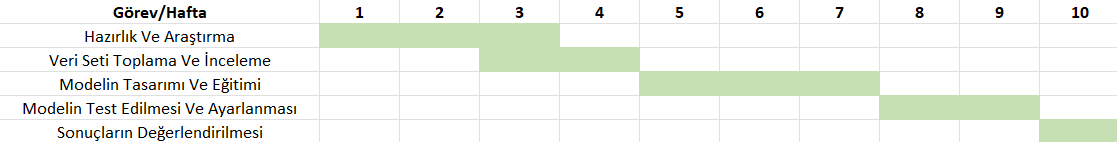
\includegraphics[width=\textwidth,height=\textheight,keepaspectratio]{Gantt .png}
  	
  		\vspace{0.7cm}
  	
  \end{figure}
  \begin{itemize}
        
      \item 
      {\bf\fontsize{12pt}{14pt}\selectfont Hazırlık ve Araştırma:} 
      RNN'ler hakkında temel bilgi edinme ve araştırma yapma, RNN'lerin gerçek hayattaki uygulamalarını inceleme,Proje kapsamı ve hedeflerinin netleştirilmesi.
      \item {\bf\fontsize{12pt}{14pt}\selectfont Veri Seti Toplama ve İnceleme:}  
      Hava durumu tahmini için uygun veri setlerini bulma ve toplama, Veri setlerini temizleme, işleme ve ön inceleme yapma.
      \item {\bf\fontsize{12pt}{14pt}\selectfont  Modelin Tasarımı ve Eğitimi:} 
      RNN modelinin mimarisini belirleme ve tasarlama,
Veri setlerini model için uygun formata dönüştürme, Modelin eğitimi için uygun algoritmaları seçme ve uygulama.
      \item {\bf\fontsize{12pt}{14pt}\selectfont  Modelin Test Edilmesi ve Ayarlanması:} 
      Eğitilen modelin performansını değerlendirme ve test etme,Modelin hata analizi yapma ve iyileştirmeler için ayarlamalar yapma, Modelin doğruluğunu artırmak için optimizasyon yöntemlerini uygulama,
      
      \item {\bf\fontsize{12pt}{14pt}\selectfont Sonuçların Değerlendirilmesi ve Raporlama:}  
      Projenin sonuçlarını derleme ve değerlendirme,
Elde edilen sonuçları raporlama ve sunum hazırlama,
Projenin başarıları, sınırlamaları ve gelecekteki çalışmalar için önerileri tartışma.
    
  \end{itemize}
  \item Kaynakça
  \begin{itemize}
  \bibitem{example} ADeep Learning Türkiye. (22 Kasım 2020). RNN Nedir? Nasıl Çalışır? Erişim tarihi: [5.03.2024].
  \url{  https://medium.com/deep-learning-turkiye/rnn-nedir-nasıl-çalışır-9e5d572689e1}
  \bibitem{example} TensorFlow. Zaman Serileri Yapılandırılmış Veri Eğitimi. Erişim tarihi: [10.03.2024]. \newline\url{https://www.tensorflow.org/tutorials/structured_data/time_series?hl=tr}
\bibitem{example} Ana Veri Sistemi.(25 Aralık 2023). Hava Durumu Ölçüm Değerleri. Erişim tarihi: [11.03.2024] \newline 
\url{ https://ulasav.csb.gov.tr/dataset/42-hava-durumu-olcum-degerleri}
\bibitem{example} Ana Veri Sistemi.(27 Mart 2023). Hava Durumu Ölçüm Değerleri. Erişim tarihi: [11.03.2024] \newline  \url{ https://ulasav.csb.gov.tr/dataset/06-hava-durumu-verileri}

  \end{itemize}


  \end{enumerate}
 
\end{document}